\chapter{线性离散系统}

\section{A/D转换}

\subsection{A/D转换}

A/D转换器将模拟信号变成数字信号。A/D转换的过程可以看作是采样、量化和编码过程

采样的过程如下图所示，假设采样开关每隔一定时间$T$闭合一次，则称$T$为采样周期，则采样频率为
\begin{center}
    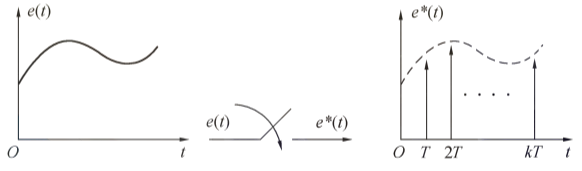
\includegraphics[width = .6\textwidth]{note/linear discrete system/figure/1.png}
\end{center}

\begin{equation*}
    f_s = \frac{1}{T}
\end{equation*}

而采样角频率为
\begin{equation*}
    \omega_s = \frac{2\pi}{T} = 2\pi f_s
\end{equation*}

采样过程可以看作是一个脉冲调制过程。设理想的单位脉冲序列为：
\begin{equation*}
    \delta_T (t) = \sum_{k=0}^\infty \delta(t-kT)
\end{equation*}

由此可以得到模拟信号的采样信号为：
\begin{equation*}
    e^* (t) = e(t) \delta_T(t) = \sum_{k=0}^\infty e(KT) \delta(t-KT)
\end{equation*}

量化就是采用有限字长的一组二进制数去逼近离散模拟信号的幅值。在计算机中，任何数值都可以表示成二进制数字量最低位的整数倍。数字量最低为所代表的数值称为量化单位通常用$q$来表示

编码就是将量化后的数值变成按某种规则编码的二进制数码。常用的编码形式有：原码，补码，偏移码、BCD码等。

\subsection{离散信号的频谱}

对于一个频谱有限连续时间信号$x(t)$，其Fourier变换为：
\begin{equation*}
    X(j\omega) = \int^\infty_{-\infty} x(t)e^{-j\omega t} dt
\end{equation*}

同样的，对于一个理想采样信号$x^* (t) = x(t) \delta_T(t) = \sum\limits_{k=0}^\infty x(KT) \delta(t-KT)$，我们可以写出他的Fourier变换：
\begin{equation*}
    X_s(\omega) = \frac{1}{2\pi} X(\omega)*(\omega_s \sum\limits_{n=-\infty}^{+\infty} \delta(\omega-n\omega_s)) = \frac{1}{T_s}\sum\limits_{n=-\infty}^{+\infty}X(\omega-n\omega_s)
\end{equation*}

考虑需要不失真地恢复原来的连续信号，理想采样角频率需要满足以下定理：

\begin{theorem}[Shannon定理]
    对于频谱有限信号$x(t)$，如果其最高频率分量为$\omega_m$，为了保留原信号的全部信息，或能无失真地恢复原信号，在通过采样得到离散信号时，其采样频率应满足$\omega_s\geq 2\omega_m$。通常把最低允许的采样频率$\omega_s = 2\omega_m$称为Nyquist频率，最大允许采样间隔$T_s = \dfrac{\pi}{\omega_m}$称为Nyquist间隔
\end{theorem}

在工程实际中，采样角频率往往取的比Nyquist频率要大得多

\subsection{采样周期的选取}

在Shannon定理中，采样周期需要越小越好，但是在工程实际中，采样周期取得过短，将会增加不必要的计算负担。反之，采样周期取得过长，又会给控制过程带来较大的误差，降低系统的动态性能

所以，根据工程实践的经验，伺服系统的采样频率可选为：
\begin{equation*}
    \omega_s \approx 10\omega_c
\end{equation*}

其中$\omega_c$为开环系统的幅值穿越频率


\section{D/A转换}
D/A转换器将数字信号转换为模拟信号。D/A转换的过程可以看成是解码和保持的过程

解码就是根据D/A转换器所采用的编码规则，将数字信号折算成对应的电压或电流值。这个电压或电流值仅仅是对应各采样时刻的，而相邻两采样时刻之间的值还没有确定。

保持就是解决各相邻采样时刻之间的插值问题，将离散时间信号变成连续时间信号。实现保持功能的器件称为保持器。保持器有各种类型，D/A转换器中一般使用零阶保持其，其传递函数通常记为$H_0(s)$。零阶保持器是一种具有常值外推功能的保持器，它将采样时刻的电压或电流值不增不减地保持到下一个采样时刻到来之前。

\section{Z变换与Z反变换}

\subsection{Z变换}

考虑一个对连续信号进行理想采样的离散信号：
\begin{equation*}
    x^* (t) = x(t) \delta_T(t) = \sum\limits_{k=0}^\infty x(KT) \delta(t-KT)
\end{equation*}

其Laplace变换为：
\begin{equation*}
    X^*(s) = \sum_{k=0}^\infty x(kT)e^{-kTs}
\end{equation*}

记复变量$z = e^{-Ts}$，则上式可以写为：
\begin{equation*}
    X(z) = \sum_{k=0}^\infty x(kT)z^{-k}
\end{equation*}

\begin{definition}
    称式子
    \begin{equation*}
    X(z) = \sum_{k=0}^\infty x(k)z^{-k}
    \end{equation*}
    为离散信号$x(k)$的Z变换，记为：$X(z) = Z[x(t)]$

    \textbf{注}：
    \begin{enumerate}
        \item     在本笔记中，记连续信号$x(t)$理想采样各个值$x(kT)$为$x(k)$，与信号分析与处理类似
        \item 默认连续信号存在Z变换，且其Z变换与其理想采样信号的Z变换相同
    \end{enumerate}


    
\end{definition}

\subsection{求Z变换的常用方法}

\subsubsection{级数求和法}

由Z变换的定义可以得到：
\begin{equation*}
    X(z) = x(0) + x(1) z^{-1} + x(2) z^{-2} + \cdots + x(k) z^{-k} +\cdots
\end{equation*}

这是$X(z)$的laurent级数表达式，故只要知道$x(k)$的闭式表达，即可求出其Z变换

\subsubsection{部分分式法}
